\chapter{Controllability and observability}\label{chap:controlandobserve}

This lab will demonstrate the fundamental ideas behind the controllability
and observability properties of a system.  You will analyze a simple circuit
and determine the conditions for observability and controllability.  You will
then proceed to simulate the system using \textsf{Simulink} under various
conditions.

\section{Background Information}

Using Figure~\ref{fig:circuit}
\begin{figure}[htbp]
    \centering
    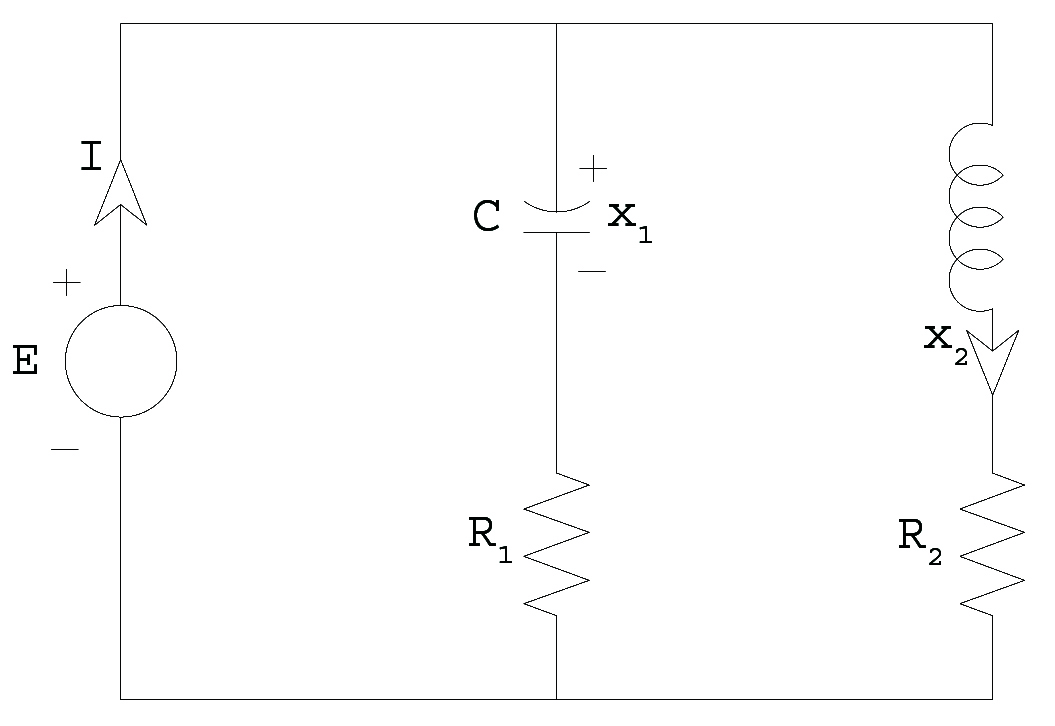
\includegraphics[width=0.6\hsize]{pix/circuitlarge.jpg}
    \caption{State space configuration}\label{fig:circuit}
\end{figure}
as a reference, define \(x_{1}\) as the voltage across the capacitor, and
\(x_{2}\) as the current through the inductor.  Take the output to be the
current entering the circuit, denoted \(I\) in Figure~\ref{fig:circuit}, and the input \(u\) to be the voltage \(E\).

We wish to write out the system equations in the state-space form:
\begin{eqnarray*}
    \dot{\vect{x}}=\mat{A}\vect{x}+\vect{b}u,\\y=\vect{c}^{t}\vect{x}+\mat{D}u.
\end{eqnarray*}
\begin{itemize}
    \item We can do this as follows.  The current through a capacitor is
          given by \(I_{c}=C\frac{dV_{C}}{dt}\), the voltage across an inductor is
          given by \(V_{L}=L\frac{dI_{L}}{dt}\), and the voltage across a resistor is
          given by Ohm's law, \(V_{R}=I_{R}R\).  By Kirchoff's voltage law, the voltage
          across each branch of the circuit is simply \(E\), which is also equal to the sum of the individual voltage drops across each branch. Then we get
          \begin{gather*}
              V_C + I_CR_1              = u \\
              V_C + C\frac{dV_C}{dt}R_1 = u \\
              \dot{x_1}                 = -\frac{1}{R_1C}x_1 + \frac{1}{R_1C}u
          \end{gather*}

          And similarly,

          \[ \dot{x_2} = -\frac{R_2}{L}x_2 + \frac{1}{L}u \]


          So we get \( \mat{A} = \begin{pmatrix}
              -\frac{1}{R_1C} & 0              \\
              0               & -\frac{R_2}{L}
          \end{pmatrix} \) and \( \mat{b} = \begin{pmatrix}
              \frac{1}{R_1C} \\ \frac{1}{L}
          \end{pmatrix} \).

    \item Since the output is the current entering the circuit, we can
          use Kirchoff's current law (i.e., conservation of current) to determine
          expressions for \(\vect{c}\) and \(\mat{D}\). In particular,
          \[ y = I_C + I_L = -\frac{1}{R_1}V_C + \frac{1}{R_1}u + I_L = \begin{pmatrix}
                  -\frac{1}{R_1} & 1
              \end{pmatrix}\vect{x} + \frac{1}{R_1}u \]
          So \( \mat{c} = \begin{pmatrix}
              -\frac{1}{R_1} \\
              1
          \end{pmatrix} \) and \( \mat{D} = \frac{1}{R_1} \).
\end{itemize}

Then, we can compute the controllability matrix \( \mat{C}(\mat{A},\vect{b}) \) as
\begin{equation}\label{eq:controlmatrix} \mat{C}(\mat{A}, \vect{b}) = \begin{pmatrix}
        \mat{b} & | & \mat{Ab}
    \end{pmatrix} = \begin{pmatrix}
        \frac{1}{R_1C} & -\frac{1}{R_1^2C^2} \\
        \frac{1}{L}    & -\frac{R_2}{L^2}
    \end{pmatrix}\end{equation}

And we can compute the observability matrix \( \mat{O}(\mat{A},\vect{c}) \) as
\begin{equation}\label{eq:observematrix} \mat{O}(\mat{A}, \vect{c}) = \begin{pmatrix}
        \mat{c}^t \\ \hline
        \mat{c}^t \mat{A}
    \end{pmatrix} = \begin{pmatrix}
        -\frac{1}{R_1}   & 1              \\
        \frac{1}{R_1^2C} & -\frac{R_2}{L}
    \end{pmatrix}\end{equation}

\section{Procedure}

First, you will determine the conditions under which the circuit in Figure~\ref{fig:circuit} is controllable and/or observable, then verify these conditions using simulation.

\begin{enumerate}
    \item \textbf{Controllability}\label{step:1}

          When analyzing the controllability, you will be examining the behaviour of
          the system states.  Recall that a rough definition of controllability is:
          ``starting from the origin, you can reach any point in state space by
          applying an appropriate input.''
          \begin{enumerate}
              \item Determine the conditions under which the system is uncontrollable, using the matrix in~\eqref{eq:controlmatrix}.
                    Recall that a square matrix has full rank if and only if its determinant is
                    non-zero.
              \item When the system is uncontrollable, determine the set of reachable
                    points for zero initial conditions (recall that the set of reachable points is related to the columnspace of \( \mat{C}(\mat{A},\vect{b}) \)). This is going to be a one-dimensional
                    vector space, so there is a simple relationship between \(x_{1}\) and \(x_{2}\).
                    Determine this relationship when the system is uncontrollable.

                    \vspace{0.5em}
                    Build the \textsf{Simulink} model as shown in
                    Figure~\ref{fig:model2}.
                    \begin{figure}[htbp]
                        \centering
                        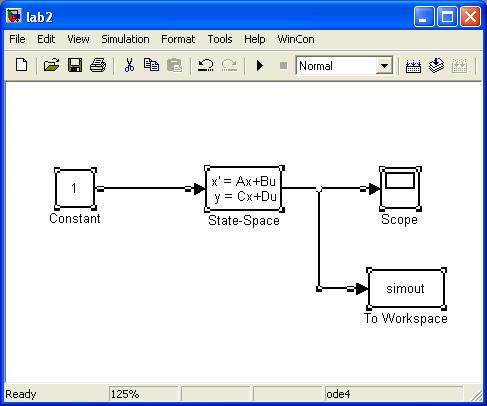
\includegraphics[width=0.6\hsize]{pix/controlandobservemodel.jpg}
                        \caption{\textsf{Simulink} model for Lab~\ref{chap:controlandobserve}}\label{fig:model2}
                    \end{figure}%
                    The model applies a constant voltage to the dynamic model defined by
                    \(\mat{A}\), \(\vect{b}\), \(\vect{c}\), and \(\mat{D}\) defined
                    previously. The output is the current in the circuit.

                    \vspace{0.5em}
                    Define the matrices \(\mat{A}$\@, \(\vect{b}$\@, \(\vect{c}\), and
                    \(\mat{D}\) by double-clicking on the \verb|State-space| block.  Each matrix is
                    entered using the following convention. The following is an example on how to
                    properly input values into the \verb|State-Space| block. The values shown are
                    \emph{not} the proper values.  Use values that correspond to the matrices in Background Information, picking your variable values to make the system controllable/uncontrollable (depending on what you're trying to simulate).  The matrix
                    \begin{equation*}
                        \mat{A}=\begin{bmatrix}0&1\\-1&2\end{bmatrix}
                    \end{equation*}
                    is entered by typing \verb|[0,1;-1,-2]| in the line reserved for \(\mat{A}$\@.
                        Note that elements of a row are delimited by comma (or spaces) and each row
                        is delimited by a semicolon.

                        \begin{figure}[htbp]
                            \centering
                            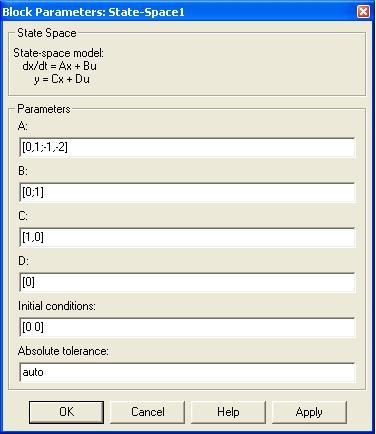
\includegraphics[width=0.6\hsize]{pix/controlandobserveentries.jpg}
                            \caption{State space configuration}\label{fig:stateConfiguration}
                        \end{figure}%
                        The entries of Figure~\ref{fig:stateConfiguration} correspond to the dynamical system
                        \begin{eqnarray*}
                            \dot{\vect{x}}&=&\begin{bmatrix}0&1\\-1&-2\end{bmatrix}\vect{x}
                            +\begin{bmatrix}0\\1\end{bmatrix}u,\\
                            y&=&\begin{bmatrix}1&0\end{bmatrix}\vect{x}+[0]u.
                        \end{eqnarray*}
                        Note that the last line specifies the initial conditions for the states.  In
                        this case, we have set \(x_{1}(0)=0\) and \(x_{2}(0)=0$\@.  Come up with an
                    appropriate variable to show the linear relationship between \(x_{1}\) and
                    \(x_{2}\) when the system is uncontrollable (make sure you record this in your
                    lab report).  Define this variable as one of your outputs in your model.
                    Note that you can add as many outputs as you want just by adding rows to the
                    matrix \(\vect{c}$\@.

                    Define the initial conditions to be zero.  The default final time is set to
                    10 by \textsf{Simulink}.  You may change it by opening the window
                    \begin{center}
                        \verb|Simulation|\(\rightarrow \)\verb|Configuration Parameters|
                    \end{center}
                    and entering the required time in the \verb|Stop Time| box.

              \item\label{step:1e} Run the \textsf{Simulink} block under uncontrollable conditions. This
                    will depend on your choice of \(R_{1}\), \(R_{2}\), \(C\), and \(L\).
                    Recuperate the state variable values written to the workspace and plot
                    \(x_{1}\), \(x_{2}\), and the output variable you defined.  Does the output
                    variable you chose show that there is, in fact, a linear relationship between
                    \(x_{1}\) and \(x_{2}\)? Under these conditions, is it possible to find an input
                    voltage \(E\) that will allow you to reach a point that is off this line? Add an appropriate title to your graph and print it.

              \item\label{step:1g} Rerun the system, but this time use conditions that make the system
                    controllable.  Plot and print a graph of \(x_{1}\) and \(x_{2}\) and your output
                    variable.  What can you now say about your output variable?  What is the set
                    of reachable points under these conditions? Again, give an appropriate title to your graph and print it.

              \item Do these plots agree with the controllability conditions you found? Explain how you can tell this from the plots.
          \end{enumerate}

    \item \textbf{Observability}\label{step:2}

          When analyzing observability, you will be examining the output behaviour of
          the system.  Recall that a rough definition of observability is: ``a change
          in initial conditions and/or input results in a change in the output.''
          \begin{enumerate}
              \item Determine the conditions under which the system is unobservable, and enter the corresponding values of \(\mat{A}\),
                    \(\vect{b}\), \(\vect{c}\), and \(\mat{D}\) into the \verb|State-Space| block.
                    Change the name of the output variable from \verb|simout| to \verb|I|.
              \item When the system is unobservable, determine the set of initial
                    conditions that yield the same output (recall that this is related to the kernel of \( \mat{O}(\mat{A},\vect{c}) \)) Find the linear relationship between
                    the initial conditions.
              \item We will want to examine the output using many different initial
                    conditions.  Build and run the system using a pair of initial conditions that
                    are in the kernel of the observability matrix.  Plot, and print a graph of
                    the output variable \(I\).  Make sure that you include values of the constants
                    in the title of the plot.
              \item Rerun the system using a different pair of initial conditions that are
                    also in the kernel of the observability matrix.  Include a plot of the
                    output. What happens if you use initial conditions that are not in the kernel
                    of the observability matrix?

              \item Do these plots agree with the observability conditions you found? Explain how you can tell this from the plots.
          \end{enumerate}

\end{enumerate}

When you have completed the lab, make sure you save your files in a convenient location (e.g.\ on some type of cloud storage).

\section{Deliverables}
Prepare a brief write up describing what you learned from this lab. This does not need to be a formal report, but all material should be presented in a clear and logical manner, with concise descriptions where necessary. Include your answers to all the questions in the lab (these are the lettered sections in the procedure), as well as any requested plots.

%%% Local Variables: 
%%% mode: latex
%%% TeX-master: "lab-manual"
%%% End: 
